\documentclass[landscape]{foils} 
\usepackage[pdftex]{graphicx}
\DeclareGraphicsExtensions{.pdf, .jpg, .tif, .png}

%\usepackage{pslatex}
\usepackage{tabularx,dcolumn, graphicx, amsfonts,amsmath}  
\usepackage[sectionbib]{natbib}
\usepackage{picinpar}
\usepackage{paralist}
\usepackage[sectionbib]{natbib}
\bibliographystyle{apalike}

\setlength{\voffset}{-0.5in}
%\setlength{\hoffset}{-0.5in}
%\setlength{\textwidth}{10.5in}
\setlength{\textheight}{7in}
\setlength{\parindent}{0pt}
%\pagestyle{empty}
%\renewcommand{\baselinestretch}{2.0}
\DeclareMathSymbol{\expect}{\mathalpha}{AMSb}{'105}
\def\p{\rm p}
\def\pp{\rm P}
\newcommand{\section}{\secdef \newsection\newsection}
\newcommand{\paup}{{\tt PAUP$^\ast$}}
%\renewcommand{\labelitemi}{\includegraphics[width=5mm]{images/bullet.pdf}}
\newcommand{\newsection}[1]{%
{
	\par\flushleft\large\sf\bfseries \vskip -2cm #1\\\rule[0.7\baselineskip]{\textwidth}{0.5mm}\par}}

\newcommand{\subsection}{\secdef \test\test}
\newcommand{\test}[1]{%
	{\par\flushleft\normalsize\sf\bfseries #1: }}
\newcommand{\M}{\mathcal{M}}
\newcommand{\prob}{{\rm Prob~}}
\def\showy#1{{\normalsize\sf\bfseries #1}}
\def\donotuse#1{}

\newcommand{\entrylabel}[1]{\mbox{#1}\hfil}
\newenvironment{entry}
	{\begin{list}{}%
		{\renewcommand{\makelabel}{\entrylabel}%
		\setlength{\labelwidth}{35pt}%
		\setlength{\leftmargin}{\labelwidth+\labelsep}%
	}%
	{\end{list}}}
% this are commands that come with the color package

\usepackage{color}
\usepackage{fancyhdr}


\pagestyle{empty}
%define colors
\definecolor{mediumblue}{rgb}{0.0509,0.35,0.568}
\definecolor{blue}{rgb}{0.0109,0.15,0.468}
\definecolor{black}{rgb}{0.04,0.06,0.2}
\definecolor{darkblue}{rgb}{0.03,0.1,0.2}
\definecolor{darkgreen}{rgb}{0.03,0.5,0.2}
\definecolor{lightblue}{rgb}{0.85,0.9333,0.95}
\definecolor{lightblue2}{rgb}{0.270588, 0.45098, 0.701961}
\definecolor{white}{rgb}{1.0,1.0,1.0}
\definecolor{yellow}{rgb}{0.961,0.972,0.047}
\definecolor{red}{rgb}{0.9,0.1,0.1}
\definecolor{orange}{rgb}{1.0,0.4,0.0}
\definecolor{violet}{rgb}{0.619608, 0.286275, 0.631373}
\definecolor{mybackgroundcolor}{rgb}{1.0,1.0,1.0}

%\definecolor{light}{rgb}{.5,0.5,0.0}
\definecolor{light}{rgb}{.3,0.3,0.3}

% sets backgroundcolor for whole document 
\pagecolor{mybackgroundcolor}
% sets text color
%\color{black}
% see below for an example how to change just a few words
% using \textcolor{color}{text}

\font \riesig=cmssbx10 scaled 13000
\font \gigant=cmssbx10 scaled 12000
\font \gross=cmssbx10 scaled 7000
\font \mittel=cmssbx10 scaled 5000
\font \courier=pcrb scaled 2000

\newcommand{\poltext}{{\copyright\ 2002--2016 by Paul O. Lewis -- Modified by  Mark Holder with permission from Paul Lewis}}

\newcommand{\pol}{{\footnotesize \poltext}}
\newcommand{\myBackground}{\begin{picture}(0,0)(0,0)  \put(-40,-70){\makebox(0,0)[l]{\includegraphics[width=33cm]{images/baby_blue.jpg}}} \end{picture}}
\newcommand{\myFooter}{}
%\begin{picture}(0,0)(0,0)
%	\put(0,-185){\pol}
%\end{picture}}
\newcommand{\myNewSlide}{\newpage\myFooter} % \myBackground}

\usepackage{url}
\usepackage{hyperref}
\hypersetup{backref,  linkcolor=black, citecolor=black, colorlinks=true, hyperindex=true}
\usepackage{pdfpages}
\begin{document}

\unitlength=1mm
 

\myNewSlide
\section*{Many types of trees: cellular genealogies}
\begin{picture}(0,0)(0,0)  
\put(-35,-55){\makebox(0,0)[l]{\includegraphics[scale=.8]{/home/mtholder/Documents/storage/talks/teaching/sisg2014/sisg2014-Mark/images/cellPhylogeny.pdf}}}
\put(120,-55){\makebox(0,0)[l]{\includegraphics[scale=.60]{/home/mtholder/Documents/storage/talks/teaching/WoodsHole2018/images/DeWittEtAlFigure1BCell.png}}}
\put(130,-135){\small Figure 1 from \href{http://matsen.fhcrc.org/papers/DeWitt2018-el.pdf}{DeWett {\em et al}. 2018}}
\end{picture}



\myNewSlide

\section*{Many types of trees:  ``gene tree'' within a species tree}
\unitlength=1mm
\begin{picture}(0,0)(0,0)  \put(-55,-70){\makebox(0,0)[l]{\includegraphics[scale=1.2]{/home/mtholder/Documents/storage/talks/teaching/sisg2014/sisg2014-Mark/images/gene_tree_sp_tree.pdf}}}
\end{picture}

\myNewSlide

\begin{picture}(150,120)(0,0)
    \put(-10,30){\includegraphics[scale=1]{/home/mtholder/Documents/storage/talks/teaching/WoodsHole2018/images/LiEcholocating2010Fig1B.png}}
     \put(100,-40){\includegraphics[scale=1]{/home/mtholder/Documents/storage/talks/teaching/WoodsHole2018/images/HahnNahklehFig2.png}}
    \put(-10, -10){Figure 1 from \cite{LiuEtAl2010}}
    \put(100, -55){Figure 2 from \cite{HahnN2016}}
\end{picture}


\myNewSlide
\section*{ Inferring a species tree while accounting for the coalescent}
\begin{picture}(150,100)(0,0)
    \put(0,-15){\includegraphics[scale=.5]{/home/mtholder/Documents/storage/talks/teaching/bodega/images/HeledD2010Fig2.png}}
    \put(0,-40){\small Figure 2 from \cite{HeledD2010} $^{\ast}$BEAST } 
    \put(0,-48){\small See also the recent work by \href{https://scholar.google.com.au/citations?hl=en&user=6m2Vc-gAAAAJ&view_op=list_works&sortby=pubdate}{Huw Ogilvie} and colleagues on StarBEAST2.} 
\end{picture}


\myNewSlide
\section*{Considering ILS effects without modeling gene trees}
\begin{picture}(150,100)(0,0)
    \put(0, 50){\color{blue}SVDQuartets }
    \put(0, 37){\color{blue}(Kubatko + Swofford}
    \put(0, 24){\color{blue} next Thursday) }
    \put(90,-10){\includegraphics[scale=.75]{/home/mtholder/Documents/storage/talks/teaching/sisg2014/sisg2014-Mark/images/PomoVsMSC-DeMaio2015Fig1.png}}
    \put(130, 100){PoMo model}
    \put(110,-35){\small Figure 1 from \cite{DeMaioSK2015}}
\end{picture}


\myNewSlide
\section*{(3a) Many types of trees: A ``gene family tree''}
\unitlength=1mm
\begin{picture}(0,0)(0,0)
  \put(-15,-60){\makebox(0,0)[l]{\includegraphics[scale=1.1]{/home/mtholder/Documents/storage/talks/teaching/sisg2014/sisg2014-Mark/images/OpazoHS2008Fig1.pdf}}}
\put(170,-55){\small Opazo, Hoffmann and Storz}
\put(170,-63){\small``Genomic evidence for}
\put(170,-71){\small independent origins of $\beta$-like}
\put(170,-79){\small globin genes in monotremes }
\put(170,-88){\small and therian mammals''}
\put(170,-97){\small PNAS {\bf 105(5)} 2008}
\end{picture}


\myNewSlide
\unitlength=1mm
\begin{picture}(0,0)(0,0)
  \put(15,-60){\makebox(0,0)[l]{\includegraphics[scale=1.2]{/home/mtholder/Documents/storage/talks/teaching/sisg2014/sisg2014-Mark/images/OpazoHS2008Fig4.pdf}}}
\put(-15,-150){\small Opazo, Hoffmann and Storz ``Genomic evidence for independent origins of $\beta$-like}
\put(-15,-158){\small globin genes in monotremes and therian mammals'' PNAS {\bf 105(5)} 2008}
\end{picture}




%%%%%%%%%%%%%%%%%%%%%%%%%%%%%%%%%%%%%%%%%%%%%%%%%%%%%%
\myNewSlide
{\bf \large  Joint estimation of gene duplication, loss, and coalescence with DLCoalRecon}\par\vskip 2em
\begin{picture}(150,100)(0,0)
    \put(0,-20){\includegraphics[scale=1.5]{/home/mtholder/Documents/storage/talks/teaching/bodega/images/RasmussenK2012Fig2a.png}}
    \put(0,-40){\small Figure 2A from \cite{RasmussenK2012}}
\end{picture}

%%%%%%%%%%%%%%%%%%%%%%%%%%%%%%%%%%%%%%%%%%%%%%%%%%%%%%
\myNewSlide
\section*{ DL models and coalescence}
\begin{picture}(150,100)(0,0)
    \put(0,-30){\includegraphics[scale=1.5]{/home/mtholder/Documents/storage/talks/teaching/bodega/images/RasmussenK2012Fig2b.png}}
    \put(0,-40){\small Figure 2B from \cite{RasmussenK2012}}
\end{picture}

\myNewSlide
\section*{Many types of trees: Lateral Gene Transfer}

{\em tree} - a graph without cycles (loops)\\
{\em network} - general graph; cycles allowed\\

Cycles can represent
\begin{compactitem}
    \item lateral (``horizontal'') gene transfer ,
    \item hybridization between species, 
    \item introgression between populations.
\end{compactitem}
\begin{picture}(50,50)(0,0)
    \put(0, 0){\includegraphics[scale=.3]{/home/mtholder/Documents/storage/talks/teaching/WoodsHole2018/images/SNaQ-logo.png}}
\end{picture}
%{\color{blue} C\'ecile An\'e (next Friday)}

\myNewSlide
\section*{Many types of trees: Lateral Gene Transfer}
\begin{picture}(150,100)(0,0)
    \put(40,-30){\includegraphics[scale=1.4]{/home/mtholder/Documents/storage/talks/teaching/bodega/images/SzollosiEtAl2013Fig2c.png}}
    \put(0,-50){\small Figure 2c from \cite{SzollosiEtAl2013}}
\end{picture}


%%%%%%%%%%%%%%%%%%%%%%%%%%%%%%%%%%%%%%%%%%%%%%%%%%%%%%
\myNewSlide
\begin{picture}(150,100)(0,0)
    \put(-10,-40){\includegraphics[scale=.8]{/home/mtholder/Documents/storage/talks/teaching/bodega/images/SzollosiEtAl2013Fig3.png}}
    \put(0,-50){\small Figure 3 from \cite{SzollosiEtAl2013}}
    \put(130,110){They used 423 single-copy genes}
    \put(130,95){in $\geq 34$ of 36 cyanobacteria}
    \put(130,70){They estimate:}
    \put(140,50){2.56 losses/family}
    \put(140,30){2.15 transfers/family}
    \put(140,10){$\approx28$\% of transfers between}
    \put(140,-10){non-overlapping branches}
\end{picture}


%%%%%%%%%%%%%%%%%%%%%%%%%%%%%%%%%%%%%%%%%%%%%%%%%%%%%%
\myNewSlide
\begin{picture}(150,100)(0,0)
    \put(20,-60){\includegraphics[scale=1.0]{/home/mtholder/Documents/storage/talks/teaching/sisg2014/sisg2014-Mark/images/NoutahiEtAl2016-figure4.png}}
    \put(0,-70){\small Figure 4 from \cite{NoutahiEtAl2016}}
\end{picture}

\myNewSlide
\section*{(3b) sources of error cartoon}
\begin{picture}(150,120)(0,0)
    \put(0,-50){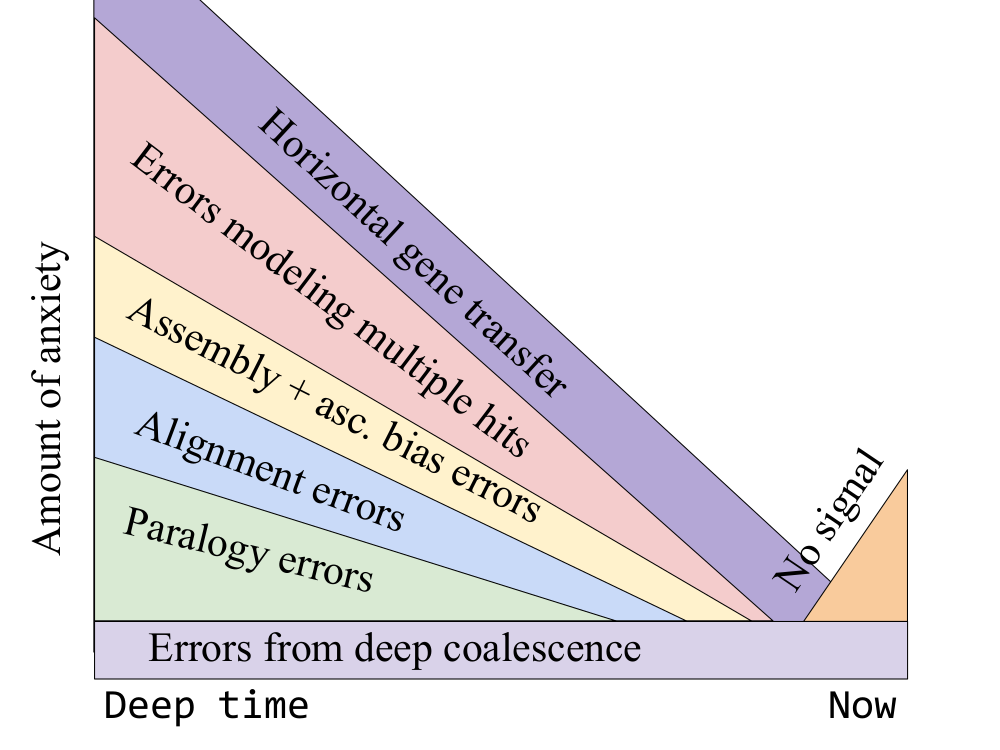
\includegraphics[scale=.9]{/home/mtholder/Documents/storage/talks/teaching/WoodsHole2018/images/source-of-bact-phylo-error-by-lookback-time.pdf}}
\end{picture}

\myNewSlide
\small
\bibliography{phylo}

\end{document}

\myNewSlide
\section*{(3c) Hypothesis testing in phylogenetics is tricky}

\begin{compactitem}
    \item complex literature on frequentists tests of topology ({\color{blue} Holder last day})
    \item bootstrapping - examining effects of sampling error using resampling via computer
    \item Bayesian methods ({\color{blue} Paul Lewis, John Huelsenbeck, Tracy Heath, and Michael Landis - this Sunday and the last Saturday})
\end{compactitem}

\includepdf[pages={1}]{/home/mtholder/Documents/storage/talks/teaching/WoodsHole/testing/newimages/JoeFelsBootFig1.pdf}
\includepdf[pages={1}]{/home/mtholder/Documents/storage/talks/teaching/WoodsHole/testing/newimages/JoeFelsBootFig2.pdf}
\includepdf[pages={1}]{/home/mtholder/Documents/storage/talks/teaching/WoodsHole/testing/newimages/JoeFelsBootFig3.pdf}

\myNewSlide
\section*{(3c) bootstrapping}

\begin{compactitem}
    \item \url{http://phylo.bio.ku.edu/mephytis/boot-sample.html}
    \item \url{http://phylo.bio.ku.edu/mephytis/bootstrap.html}
\end{compactitem}

\myNewSlide
\section*{(3d) Phylogenetics is computationally difficult}
Problems:
\begin{compactitem}
    \item Huge number of trees
    \item Strange geometry of tree space
    \item Large number of numerical parameters that need to be considered.
\end{compactitem}
Some strategies:
\begin{compactitem}
    \item Pragmatic computational heuristics for tree searching 
    -- {\color{blue} Emily Jane McTavish (tomorrow) and
    Bui Quang Minh (Tuesday)}
    \item Markov chain Monte Carlo ({\color{blue} Paul Lewis, John Huelsenbeck, Tracy Heath, and Michael Landis - this Sunday and the last Saturday})
\end{compactitem}





\myNewSlide
\section*{Optimality criteria}
A rule for ranking trees (according to the data).\\
Each criterion produces a score.\par
Examples:
\begin{itemize}
    \item Parsimony (Maximum Parsimony, MP)
    \item Maximum Likelihood (ML)
    \item Minimum Evolution (ME)
    \item Least Squares (LS)
\end{itemize}

\myNewSlide
\begin{tabular}{lcccccccccccc}
 &1&2&3&4&5&6&7&8&9&.&.&.\\
 Species 1\hskip 2mm& C & G  & A & C & C & {\bf A }& G & G & T &.&.&.\\
 Species 2\hskip 2mm& C & G  & A & C & C &  {\bf A }& G & G & T &.&.&.\\
 Species 3\hskip 2mm& C & G  & G & T & C &  {\bf C }& G & G & T &.&.&.\\
 Species 4\hskip 2mm& C & G  & G & C & C & {\bf  T }& G & G & T &.&.&.\\
\end{tabular}

\vskip 8em
{\footnotesize next few slides from Paul Lewis}
\myNewSlide

\begin{tabular}{lcccccccccccc}
 &1&2&3&4&5&6&7&8&9&.&.&.\\
 Species 1\hskip 2mm& C & G  & A & C & C & {\bf A }& G & G & T &.&.&.\\
 Species 2\hskip 2mm& C & G  & A & C & C &  {\bf A }& G & G & T &.&.&.\\
 Species 3\hskip 2mm& C & G  & G & T & C &  {\bf C }& G & G & T &.&.&.\\
 Species 4\hskip 2mm& C & G  & G & C & C & {\bf  T }& G & G & T &.&.&.\\
\end{tabular}

\begin{picture}(0,0)(0,0)  
\put(0,-80){\makebox(0,0)[l]{\includegraphics[scale=1.2]{/home/mtholder/Documents/storage/talks/teaching/sisg2014/sisg2014-Mark/images/simple_unrooted.pdf}}}
\put(-10,-60){Species 1}
\put(-10,-110){Species 2}
\put(50,-60){Species 3}
\put(50,-110){Species 4}
\put(-10, -45){\normalsize One of the 3 possible trees:}
\end{picture}

\myNewSlide

\begin{tabular}{lcccccccccccc}
 &1&2&3&4&5&6&7&8&9&.&.&.\\
 Species 1\hskip 2mm& C & G  & A & C & C & {\bf A }& G & G & T &.&.&.\\
 Species 2\hskip 2mm& C & G  & A & C & C &  {\bf A }& G & G & T &.&.&.\\
 Species 3\hskip 2mm& C & G  & G & T & C &  {\bf C }& G & G & T &.&.&.\\
 Species 4\hskip 2mm& C & G  & G & C & C & {\bf  T }& G & G & T &.&.&.\\
\end{tabular}

\begin{picture}(0,0)(0,0)  
\put(0,-80){\makebox(0,0)[l]{\includegraphics[scale=1.2]{/home/mtholder/Documents/storage/talks/teaching/sisg2014/sisg2014-Mark/images/simple_unrooted.pdf}}}
\put(-10,-60){Species 1}
\put(-10,-110){Species 2}
\put(50,-60){Species 3}
\put(50,-110){Species 4}
\put(-10, -45){\normalsize One of the 3 possible trees:}
\put(120,-80){\makebox(0,0)[l]{\includegraphics[scale=1.2]{/home/mtholder/Documents/storage/talks/teaching/sisg2014/sisg2014-Mark/images/simple_unrooted.pdf}}}
\put(115,-60){A}
\put(115,-110){A}
\put(185,-60){C}
\put(185,-110){T}
\put(110, -35){\normalsize Same tree with states at character 6}
\put(110, -45){\normalsize instead of species names}
\end{picture}

\myNewSlide
\section*{Unordered Parsimony}
\begin{picture}(0,0)(0,0)  
\put(-7,-70){\makebox(0,0)[l]{\includegraphics[scale=1.1]{/home/mtholder/Documents/storage/talks/teaching/sisg2014/sisg2014-Mark/images/standard_pars_all_recon.pdf}}}
\end{picture}

\myNewSlide
\section*{Things to note about the last slide}
\large
\begin{itemize}
	\item 2 steps was the minimum score attainable.
	\item Multiple ancestral character state reconstructions gave a score of 2.
	\item Enumeration of all possible ancestral character states is {\bf  not} the most efficient algorithm.
\end{itemize}

\myNewSlide
\section*{Each character (site) is assumed to be independent}
To calculate the parsimony score for a tree we simply sum the scores for every site.
\vskip 2mm

\begin{tabular}{lccccccccc}
 &1&2&3&4&5&6&7&8&9\\
 Species 1\hskip 2mm& C & G  & {\bf A} & C & C & A & G & G & T \\
 Species 2\hskip 2mm& C & G  & {\bf A}& C & C &  A & G & G & T \\
 Species 3\hskip 2mm& C & G  & {\bf G}& T & C & C & G & G & T \\
 Species 4\hskip 2mm& C & G  & {\bf G }& C & C & T & G & G & T \\
\hline
Score\hskip 2mm& 0 & 0  & {\bf 1} & 1 & 0 & 2& 0 & 0& 0\\
\end{tabular}\\
\begin{picture}(0,0)(0,0)  
\put(80,-33){\makebox(0,0)[l]{\includegraphics[scale=1.2]{/home/mtholder/Documents/storage/talks/teaching/sisg2014/sisg2014-Mark/images/simple_unrooted.pdf}}}
\put(60,-10){Species 1}
\put(60,-60){Species 2}
\put(130,-10){Species 3}
\put(130,-60){Species 4}
\put(160, -35){Tree 1 has a score of {\bf 4}}
\end{picture}  

\myNewSlide
\section*{Considering a different tree}
We can repeat the scoring for each tree.
\vskip 2mm

\begin{tabular}{lccccccccc}
 &1&2&3&4&5&6&7&8&9\\
 Species 1\hskip 2mm& C & G  & {\bf A} & C & C & A & G & G & T \\
 Species 2\hskip 2mm& C & G  & {\bf A}& C & C &  A & G & G & T \\
 Species 3\hskip 2mm& C & G  & {\bf G}& T & C & C & G & G & T \\
 Species 4\hskip 2mm& C & G  & {\bf G }& C & C & T & G & G & T \\
\hline
Score\hskip 2mm& 0 & 0  & {\bf 2} & 1 & 0 & 2& 0 & 0& 0\\
\end{tabular}\\
\begin{picture}(0,0)(0,0)  
\put(80,-38){\makebox(0,0)[l]{\includegraphics[scale=1.2]{/home/mtholder/Documents/storage/talks/teaching/sisg2014/sisg2014-Mark/images/simple_unrooted.pdf}}}
\put(60,-15){Species 1}
\put(60,-65){Species 3}
\put(130,-15){Species 2}
\put(130,-65){Species 4}
\put(160, -40){Tree 2 has a score of {\bf 5}}
\end{picture}  

\myNewSlide
\section*{One more tree}
Tree 3 has the same score as tree 2
\vskip 2mm

\begin{tabular}{lccccccccc}
 &1&2&3&4&5&6&7&8&9\\
 Species 1\hskip 2mm& C & G  & {\bf A} & C & C & A & G & G & T \\
 Species 2\hskip 2mm& C & G  & {\bf A}& C & C &  A & G & G & T \\
 Species 3\hskip 2mm& C & G  & {\bf G}& T & C & C & G & G & T \\
 Species 4\hskip 2mm& C & G  & {\bf G }& C & C & T & G & G & T \\
\hline
Score\hskip 2mm& 0 & 0  & {\bf 2} & 1 & 0 & 2& 0 & 0& 0\\
\end{tabular}\\
\begin{picture}(0,0)(0,0)  
\put(80,-38){\makebox(0,0)[l]{\includegraphics[scale=1.2]{/home/mtholder/Documents/storage/talks/teaching/sisg2014/sisg2014-Mark/images/simple_unrooted.pdf}}}
\put(60,-15){Species 1}
\put(60,-65){Species 4}
\put(130,-15){Species 2}
\put(130,-65){Species 3}
\put(160, -40){Tree 3 has a score of {\bf 5}}
\end{picture}  

\myNewSlide
\section*{Parsimony criterion prefers tree 1}
Tree 1 required the {\em fewest} number of state changes (DNA substitutions) to explain the data.\par
Some parsimony advocates equate the preference for the fewest number of changes to the general scientific principle of preferring the simplest explanation (Ockham's Razor), but this connection has not been made in a rigorous manner.
\myNewSlide
\section*{Parsimony terms}
\begin{itemize}
	\item {\em homoplasy} multiple acquisitions of the same character state
	\begin{itemize}
		\item parallelism, reversal, convergence
		\item recognized by a tree requiring more than the minimum number of steps
		\item minimum number of steps is the number of observed states minus 1
	\end{itemize}
\end{itemize}
The parsimony criterion is equivalent to minimizing homoplasy.

Homoplasy is one form of the multiple hits problem. In pop-gen terms, it is a violation of the infinite-alleles model.
%
%\myNewSlide
%\section*{Parsimony terms}
%\begin{itemize}
%	\item {\em apomorphy }-- a derived (newly acquired) character state
%	\item {\em plesiomorphy }-- the ancestral character state
%\end{itemize}
%\begin{picture}(0,0)(0,0)  
%\put(80,-38){\makebox(0,0)[l]{\includegraphics[scale=.8]{/home/mtholder/Documents/storage/talks/teaching/sisg2014/sisg2014-Mark/images/apo_pleiso_morphy.pdf}}}
%\end{picture}

\myNewSlide
In the example matrix at the beginning of these slides, only character 3 is parsimony informative.\par
\begin{tabular}{lccccccccc}
 &1&2&3&4&5&6&7&8&9\\
 Species 1\hskip 2mm& C & G  & {\bf A} & C & C & A & G & G & T \\
 Species 2\hskip 2mm& C & G  & {\bf A}& C & C &  A & G & G & T \\
 Species 3\hskip 2mm& C & G  & {\bf G}& T & C & C & G & G & T \\
 Species 4\hskip 2mm& C & G  & {\bf G }& C & C & T & G & G & T \\
\hline
Max score\hskip 2mm& 0 & 0  & {\bf 2} & 1 & 0 & 2& 0 & 0& 0\\
Min score\hskip 2mm& 0 & 0  & {\bf 1} & 1 & 0 & 2& 0 & 0& 0\\
\end{tabular}


% \myNewSlide
% \section*{Assumptions about the evolutionary process can be incorporated using different step costs}
% \begin{picture}(0,0)(0,0)  
% \put(40,-30){\makebox(0,0)[l]{\includegraphics[scale=.8]{/home/mtholder/Documents/storage/talks/teaching/sisg2014/sisg2014-Mark/images/wag_fitch.pdf}}}
% \put(120, -60){Fitch Parsimony}
% \put(130, -70){``unordered''}
% \end{picture}

% \myNewSlide
% \section*{Stepmatrices}
% \begin{center}
% Fitch Parsimony Stepmatrix\par
% \begin{tabular}{lcccccc}
% & & & &To & \\
% & &\vline & A \hskip 2mm  &C  \hskip 2mm &G \hskip 2mm &  T\hskip 2mm\\
% \hline & A \hskip 2mm & \vline & 0 &1 & 1 &  1\\
% From &C \hskip 2mm &\vline  & 1 & 0 &1 & 1 \\
% &G \hskip 2mm &\vline  &1 & 1 & 0  & 1 \\
% &T \hskip 2mm &\vline  &1 & 1 & 1 & 0   \\
% \end{tabular}
% \end{center}
% \myNewSlide

% \section*{Stepmatrices}
% \begin{center}
% \large
% Transversion-Transition 5:1 Stepmatrix\par
% \begin{tabular}{lcccccc}
% & & & &To & \\
% & &\vline & A \hskip 2mm  &C  \hskip 2mm &G \hskip 2mm &  T\hskip 2mm\\
% \hline & A \hskip 2mm & \vline & 0 &5 & 1 &  5\\
% From &C \hskip 2mm &\vline  & 5 & 0 &5 & 1 \\
% &G \hskip 2mm &\vline  &1 & 5 & 0  & 5 \\
% &T \hskip 2mm &\vline  &5 & 1 & 5 & 0   \\
% \end{tabular}
% \end{center}

% \myNewSlide
% \section*{5:1 Transversion:Transition parsimony}
% \begin{picture}(0,0)(0,0)  
% \put(-7,-70){\makebox(0,0)[l]{\includegraphics[scale=1.1]{/home/mtholder/Documents/storage/talks/teaching/sisg2014/sisg2014-Mark/images/5to1_transversion_all_recon.pdf}}}
% \end{picture}

% \myNewSlide
% \section*{Stepmatrix considerations}
% \begin{itemize}
% 	\item Parsimony scores from different stepmatrices cannot be meaningfully compared (31 under Fitch is not ``better'' than 45 under a transversion:transition stepmatrix)
% 	\item Parsimony cannot be used to infer the stepmatrix weights
% \end{itemize}

% \myNewSlide
% \section*{Other Parsimony variants}
% \begin{itemize}
% 	\item {\em Dollo} derived state can only arise once, but reversals can be frequent ({\em e.g.} restriction enzyme sites).
% 	\item ``weighted'' - usually means that different characters are weighted differently (slower, more reliable characters usually given higher weights).
% 	\item implied weights \citet{Goloboff1993}
% \end{itemize}

% \myNewSlide
% \section*{Scoring trees under parsimony is fast}
% \begin{picture}(0,0)(0,0)  
% \put(50,-70){\makebox(0,0)[l]{\includegraphics[scale=1.1]{/home/mtholder/Documents/storage/talks/teaching/sisg2014/sisg2014-Mark/images/simple_tree.pdf}}}
% \Large
% \put(45, -15){A}
% \put(67, -15){C}
% \put(92, -15){C}
% \put(120, -15){A}
% \put(136, -15){A}
% \put(166, -15){G}
% \end{picture}

% \myNewSlide
% \section*{Scoring trees under parsimony is fast  -- Fitch algorithm}
% \begin{picture}(0,0)(0,0)  
% \put(50,-70){\makebox(0,0)[l]{\includegraphics[scale=1.1]{/home/mtholder/Documents/storage/talks/teaching/sisg2014/sisg2014-Mark/images/simple_tree.pdf}}}
% \Large
% \put(45, -15){A}
% \put(67, -15){C}
% \put(92, -15){C}
% \put(120, -15){A}
% \put(136, -15){A}
% \put(166, -15){G}
% \put(117, -38){\large \{A,C\}}
% \put(122, -49){\large +1}
% \put(160, -38){\large \{A,G\}}
% \put(162, -49){\large +1}
% \put(135, -80){\large \{A\}}
% \put(125, -97){\large \{A, C\}}
% \put(127, -108){\large +1}
% \put(110, -125){\large\{A\}}
% \put(10, -70){\Large 3 steps}
% \end{picture}

% \myNewSlide
% \section*{Scoring trees under parsimony is fast}
% The ``down-pass state sets'' calculated in the Fitch algorithm can be stored at an internal node.

% This lets you treat those internal nodes as pseudo-tips:
% \begin{compactitem}
% 	\item avoid rescoring the entire tree if you make a small change, and
% 	\item break up the tree into smaller subtrees (Goloboff's sectorial searching).
% \end{compactitem}

\myNewSlide
\section*{Qualitative description of parsimony}
\begin{compactitem}
	\item Enables estimation of ancestral sequences.
	\item Even though parsimony always seeks to minimizes the number of changes, it can perform well even when changes are not rare. 
	\item Does not ``prefer'' to put changes on one branch over another
	\item Hard to characterize statistically
	\begin{compactitem}
		\item the set of conditions in which parsimony is guaranteed to work well is very restrictive (low probability of change and not too much branch length heterogeneity);
	   \item Parsimony often performs well in simulation studies (even when outside the zones in which it is guaranteed to work); 
	   	\item Estimates of the tree can be extremely biased.
	\end{compactitem}	   
\end{compactitem}

\myNewSlide
\section*{Long branch attraction}
\begin{picture}(0,0)(0,0)  
\put(20,-60){\makebox(0,0)[l]{\includegraphics[scale=1.1]{/home/mtholder/Documents/storage/talks/teaching/sisg2014/sisg2014-Mark/images/fels_tree.pdf}}}
\put(100, -0){\normalsize Felsenstein, J. 1978. Cases in which}
\put(100, -10){\normalsize  parsimony or compatibility methods will be}
\put(100, -20){\normalsize positively misleading. {\em Systematic Zoology}}
\put(100, -30){\normalsize {\bf 27}: 401-410.}
\put(20, -50){\small 1.0}
\put(68, -50){\small 1.0}
\put(44, -120){\small 0.01}
\put(55, -115){\small 0.01}
\put(30, -115){\small 0.01}
\end{picture}

\myNewSlide
\section*{Long branch attraction}
\begin{picture}(0,0)(0,0)  
\put(20,-60){\makebox(0,0)[l]{\includegraphics[scale=1.1]{/home/mtholder/Documents/storage/talks/teaching/sisg2014/sisg2014-Mark/images/fels_tree.pdf}}}
\put(38,-103){\makebox(0,0)[l]{\includegraphics[scale=1]{/home/mtholder/Documents/storage/talks/teaching/sisg2014/sisg2014-Mark/images/lightning.pdf}}}
\put(100, -0){\normalsize Felsenstein, J. 1978. Cases in which}
\put(100, -10){\normalsize  parsimony or compatibility methods will be}
\put(100, -20){\normalsize positively misleading. {\em Systematic Zoology}}
\put(100, -30){\normalsize {\bf 27}: 401-410.}
\put(100, -60){\normalsize The probability of a parsimony informative}
\put(100, -70){\normalsize site due to inheritance is very low,}
 \put(100, -80){\normalsize (roughly 0.0003).}
\put(16, -0){\large A}
\put(75, -0){\large G}
\put(35, -123){\large A}
\put(56, -123){\large G}
\put(20, -50){\small 1.0}
\put(68, -50){\small 1.0}
\put(44, -120){\small 0.01}
\put(55, -115){\small 0.01}
\put(30, -115){\small 0.01}
\end{picture}

\myNewSlide
\section*{Long branch attraction}
\begin{picture}(0,0)(0,0)  
\put(20,-60){\makebox(0,0)[l]{\includegraphics[scale=1.1]{/home/mtholder/Documents/storage/talks/teaching/sisg2014/sisg2014-Mark/images/fels_tree.pdf}}}
\put(50,-50){\rotatebox{90}{\includegraphics{/home/mtholder/Documents/storage/talks/teaching/sisg2014/sisg2014-Mark/images/lightning.pdf}}}
\put(10,-50){\rotatebox{90}{\includegraphics{/home/mtholder/Documents/storage/talks/teaching/sisg2014/sisg2014-Mark/images/lightning.pdf}}}
\put(100, -0){\normalsize Felsenstein, J. 1978. Cases in which}
\put(100, -10){\normalsize  parsimony or compatibility methods will be}
\put(100, -20){\normalsize positively misleading. {\em Systematic Zoology}}
\put(100, -30){\normalsize {\bf 27}: 401-410.}
\put(100, -60){\normalsize The probability of a parsimony informative}
\put(100, -70){\normalsize site due to inheritance is very low,}
\put(100, -80){\normalsize (roughly 0.0003).}
\put(100, -100){\normalsize The probability of a misleading parsimony}
\put(100, -110){\normalsize informative site due to parallelism is much}
\put(100, -120){\normalsize higher (roughly 0.008).}
\put(16, -0){\large A}
\put(75, -0){\large A}
\put(35, -123){\large G}
\put(56, -123){\large G}
\put(20, -50){\small 1.0}
\put(68, -50){\small 1.0}
\put(44, -120){\small 0.01}
\put(55, -115){\small 0.01}
\put(30, -115){\small 0.01}
\end{picture}

\myNewSlide
\section*{Long branch attraction}
Parsimony is almost guaranteed to get this tree wrong.\\
\begin{picture}(0,0)(0,0)  
\put(20,-60){\makebox(0,0)[l]{\includegraphics[scale=1.1]{/home/mtholder/Documents/storage/talks/teaching/sisg2014/sisg2014-Mark/images/fels_tree.pdf}}}
\put(120,-60){\makebox(0,0)[l]{\includegraphics[scale=1.1]{/home/mtholder/Documents/storage/talks/teaching/sisg2014/sisg2014-Mark/images/inferred_fels.pdf}}}
\put(16, -0){\large 1}
\put(75, -0){\large 3}
\put(35, -123){\large 2}
\put(56, -123){\large 4}
\put(42, -133){\large True}
\put(115, -20){\large 1}
\put(200, -20){\large 3}
\put(150, -103){\large 2}
\put(165, -103){\large 4}
\put(152, -123){\large Inferred}
\end{picture}

\myNewSlide
\section*{Inconsistency}
\begin{itemize}	
	\item Statistical Consistency (roughly speaking) is converging to the true answer as the amount of data goes to $\infty$.
	\item Parsimony based tree inference is {\em not} consistent for some tree shapes.  In fact it can be ``positively misleading'':
	 \begin{itemize}	
		\item ``Felsenstein zone'' tree
		\item Many clocklike trees with short internal branch lengths and long terminal branches (Penny {\em et al.}, 1989, Huelsenbeck and Lander, 2003).
	\end{itemize}
	\item Methods for assessing confidence (e.g. bootstrapping) will indicate that you should be very confident in the wrong answer.
\end{itemize}



% \myNewSlide
% \section*{Parsimony terms}
% \begin{itemize}
% 	\item {\em synapomorphy }-- a {\sf shared} derived (newly acquired) character state.  Evidence of monophletic groups.
% \end{itemize}
% \begin{picture}(0,0)(0,0)  
% \put(60,-45){\makebox(0,0)[l]{\includegraphics[scale=.8]{/home/mtholder/Documents/storage/talks/teaching/sisg2014/sisg2014-Mark/images/apo_pleiso_morphy.pdf}}}
% \end{picture}
% \myNewSlide
% \section*{Parsimony terms}
% \begin{itemize}
% 	\item {\em parsimony informative }-- a character with parsimony score variation across trees 
% 	\begin{itemize}
% 		\item {\em min} score $\neq$ {\em max} score
% 		\item must be variable.
% 		\item must have more than one {\em shared} state
% 	\end{itemize}
% \end{itemize}

% \myNewSlide
% \section*{Consistency Index (CI)}
% \begin{itemize}
% 	\item minimum number of changes divided by the number required on the tree.
% 	\item CI=1 if there is no homoplasy
% 	\item negatively correlated with the number of species sampled
% \end{itemize}

% \myNewSlide
% \section*{Retention Index (RI)}
%  \[\mbox{RI} = \frac{\mbox{MaxSteps}-\mbox{ObsSteps}}{\mbox{MaxSteps}-\mbox{MinSteps}}\] 
% \begin{itemize}
% 	\item defined to be 0 for parsimony uninformative characters
% 	\item RI=1 if the character fits perfectly
% 	\item RI=0 if the tree fits the character as poorly as possible
% \end{itemize}


% \myNewSlide
% \section*{Transversion parsimony}
% \begin{itemize}
% 	\item Transitions ($A\leftrightarrow G$, $C\leftrightarrow T$) occur more frequently than transversions (purine $\leftrightarrow$ pyrimidine)
% 	\item So, {\em homoplasy} involving transitions is much more common than transversions ({\em e.g.} $A\rightarrow G \rightarrow A$)
% 	\item Transversion parsimony (also called $RY$-coding) ignores all transitions
% \end{itemize}

% \myNewSlide
% \section*{Transversion parsimony}
% \begin{picture}(0,0)(0,0)  
% \put(-7,-70){\makebox(0,0)[l]{\includegraphics[scale=1.1]{/home/mtholder/Documents/storage/talks/teaching/sisg2014/sisg2014-Mark/images/transversion_all_recon.pdf}}}
% \end{picture}


\myNewSlide

\section*{Long branch attraction tree again}
\begin{picture}(0,0)(0,0)  
\put(20,-60){\makebox(0,0)[l]{\includegraphics[scale=1.1]{/home/mtholder/Documents/storage/talks/teaching/sisg2014/sisg2014-Mark/images/fels_tree.pdf}}}
\put(100, -60){\normalsize The probability of a parsimony informative}
\put(100, -70){\normalsize site due to inheritance is very low,}
\put(100, -80){\normalsize (roughly 0.0003).}
\put(100, -100){\normalsize The probability of a misleading parsimony}
\put(100, -110){\normalsize informative site due to parallelism is much}
\put(100, -120){\normalsize higher (roughly 0.008).}
\put(16, -0){\large 1}
\put(75, -0){\large 4}
\put(35, -123){\large 2}
\put(56, -123){\large 3}
\put(20, -50){\small 1.0}
\put(68, -50){\small 1.0}
\put(44, -120){\small 0.01}
\put(55, -115){\small 0.01}
\put(30, -115){\small 0.01}
\end{picture}

\myNewSlide
\Large
If the data is generated such that:

\begin{eqnarray*}
\Pr
\left(
\begin{array}{c}
 A \\
 A \\
 G \\   
 G 
\end{array}
\right)\approx 0.0003 &\mbox{and} & \Pr
\left(
\begin{array}{c}
 A \\
 G \\
 G \\   
 A 
\end{array}
\right) \approx 0.008
\end{eqnarray*}
then how can we hope to infer the tree ((1,2),3,4) ?

\myNewSlide
\Large
Note:
((1,2),3,4) is referred to as Newick or New Hampshire notation for the tree.

You can read it by following the rules:
\begin{compactitem}
	\item start at a node,
	\item if the next symbol is `(' then add a child to the current node and move to this child,
	\item if the next symbol is a label, then label the node that you are at,
	\item if the next symbol is a comma, then move back to the current node's parent and add another child,
	\item if the next symbol is a `)', then move back to the current node's parent.
\end{compactitem}

% \myNewSlide
% ((1,2),3,4)

% \begin{picture}(0,0)(20,20)
% 	\thicklines
% 	\put(150,-50){\circle*{3}}
% \end{picture}

% \myNewSlide
% \Large
% {\color{red}(}(1,2),3,4)

% \begin{picture}(0,0)(20,20)
% 	\thicklines
% 	\put(150,-50){\circle*{3}}
% 	\thicklines
% 	\put(150,-50){\color{red}{\line(-1,1){30}}}
% 	\put(120,-20){\color{red}{\circle*{3}}}
% \end{picture}


% \myNewSlide
% \Large
% ({\color{red}(}1,2),3,4)

% \begin{picture}(0,0)(20,20)
% 	\thicklines
% 	\put(150,-50){\circle*{3}}
% 	\thicklines
% 	\put(150,-50){{\line(-1,1){30}}}
% 	\put(120,-20){{\circle*{3}}}
% 	\put(120,-20){\color{red}{\line(-1,1){30}}}
% 	\put(90,10){\color{red}{\circle*{3}}}
% \end{picture}

% \myNewSlide
% \Large
% (({\color{red}1},2),3,4)

% \begin{picture}(0,0)(20,20)
% 	\thicklines
% 	\put(150,-50){\circle*{3}}
% 	\thicklines
% 	\put(150,-50){{\line(-1,1){30}}}
% 	\put(120,-20){{\circle*{3}}}
% 	\put(120,-20){{\line(-1,1){30}}}
% 	\put(90,10){{\circle*{3}}}
% 	\put(85,15){\color{red}1}
% \end{picture}

% \myNewSlide
% \Large
% ((1{\color{red},}2),3,4)

% \begin{picture}(0,0)(20,20)
% 	\thicklines
% 	\put(150,-50){\circle*{3}}
% 	\thicklines
% 	\put(150,-50){{\line(-1,1){30}}}
% 	\put(120,-20){{\circle*{3}}}
% 	\put(120,-20){{\line(-1,1){30}}}
% 	\put(90,10){{\circle*{3}}}
% 	\put(87,15){1}
% 	\put(120,-20){\color{red}{\line(1,1){30}}}
% 	\put(150,10){\color{red}{\circle*{3}}}
% \end{picture}

% \myNewSlide
% \Large
% ((1,{\color{red}2}),3,4)

% \begin{picture}(0,0)(20,20)
% 	\thicklines
% 	\put(150,-50){\circle*{3}}
% 	\thicklines
% 	\put(150,-50){{\line(-1,1){30}}}
% 	\put(120,-20){{\circle*{3}}}
% 	\put(120,-20){{\line(-1,1){30}}}
% 	\put(90,10){{\circle*{3}}}
% 	\put(87,15){1}
% 	\put(120,-20){{\line(1,1){30}}}
% 	\put(150,10){{\circle*{3}}}
% 	\put(147,15){\color{red}2}
% \end{picture}

% \myNewSlide
% \Large
% ((1,2{\color{red})},3,4)

% \begin{picture}(0,0)(20,20)
% 	\thicklines
% 	\put(150,-50){\circle*{3}}
% 	\thicklines
% 	\put(150,-50){{\line(-1,1){30}}}
% 	\put(120,-20){{\line(-1,1){30}}}
% 	\put(90,10){{\circle*{3}}}
% 	\put(87,15){1}
% 	\put(120,-20){{\line(1,1){30}}}
% 	\put(150,10){{\circle*{3}}}
% 	\put(120,-20){\color{red}{\circle*{3}}}
% 	\put(147,15){2}
% \end{picture}

% \myNewSlide
% \Large
% ((1,2){\color{red},}3,4)

% \begin{picture}(0,0)(20,20)
% 	\thicklines
% 	\put(150,-50){\circle*{3}}
% 	\thicklines
% 	\put(150,-50){{\line(-1,1){30}}}
% 	\put(120,-20){{\circle*{3}}}
% 	\put(120,-20){{\line(-1,1){30}}}
% 	\put(90,10){{\circle*{3}}}
% 	\put(87,15){1}
% 	\put(120,-20){{\line(1,1){30}}}
% 	\put(150,10){{\circle*{3}}}
% 	\put(147,15){2}
% 	\put(150,-50){\color{red}{\line(0,1){30}}}
% 	\put(150,-20){\color{red}{\circle*{3}}}
% \end{picture}

% \myNewSlide
% \Large
% ((1,2),{\color{red}3},4)

% \begin{picture}(0,0)(20,20)
% 	\thicklines
% 	\put(150,-50){\circle*{3}}
% 	\thicklines
% 	\put(150,-50){{\line(-1,1){30}}}
% 	\put(120,-20){{\circle*{3}}}
% 	\put(120,-20){{\line(-1,1){30}}}
% 	\put(90,10){{\circle*{3}}}
% 	\put(87,15){1}
% 	\put(120,-20){{\line(1,1){30}}}
% 	\put(150,10){{\circle*{3}}}
% 	\put(147,15){2}
% 	\put(150,-50){{\line(0,1){30}}}
% 	\put(150,-20){{\circle*{3}}}
% 	\put(147,-15){\color{red}3}
% \end{picture}

% \myNewSlide
% \Large
% ((1,2),3{\color{red},}4)

% \begin{picture}(0,0)(20,20)
% 	\thicklines
% 	\put(150,-50){\circle*{3}}
% 	\thicklines
% 	\put(150,-50){{\line(-1,1){30}}}
% 	\put(120,-20){{\circle*{3}}}
% 	\put(120,-20){{\line(-1,1){30}}}
% 	\put(90,10){{\circle*{3}}}
% 	\put(87,15){1}
% 	\put(120,-20){{\line(1,1){30}}}
% 	\put(150,10){{\circle*{3}}}
% 	\put(147,15){2}
% 	\put(150,-50){{\line(0,1){30}}}
% 	\put(150,-20){{\circle*{3}}}
% 	\put(147,-15){3}
% 	\put(150,-50){\color{red}{\line(1,1){30}}}
% 	\put(180,-20){\color{red}{\circle*{3}}}
% \end{picture}

% \myNewSlide
% \Large
% ((1,2),3,{\color{red}4})

% \begin{picture}(0,0)(20,20)
% 	\thicklines
% 	\put(150,-50){\circle*{3}}
% 	\thicklines
% 	\put(150,-50){{\line(-1,1){30}}}
% 	\put(120,-20){{\circle*{3}}}
% 	\put(120,-20){{\line(-1,1){30}}}
% 	\put(90,10){{\circle*{3}}}
% 	\put(87,15){1}
% 	\put(120,-20){{\line(1,1){30}}}
% 	\put(150,10){{\circle*{3}}}
% 	\put(147,15){2}
% 	\put(150,-50){{\line(0,1){30}}}
% 	\put(150,-20){{\circle*{3}}}
% 	\put(147,-15){3}
% 	\put(150,-50){{\line(1,1){30}}}
% 	\put(180,-20){{\circle*{3}}}
% 	\put(177,-15){\color{red}4}
% \end{picture}

% \myNewSlide
% \Large
% ((1,2),3,4{\color{red})}

% \begin{picture}(0,0)(20,20)
% 	\thicklines
% 	\thicklines
% 	\put(150,-50){{\line(-1,1){30}}}
% 	\put(120,-20){{\circle*{3}}}
% 	\put(120,-20){{\line(-1,1){30}}}
% 	\put(90,10){{\circle*{3}}}
% 	\put(87,15){1}
% 	\put(120,-20){{\line(1,1){30}}}
% 	\put(150,10){{\circle*{3}}}
% 	\put(147,15){2}
% 	\put(150,-50){{\line(0,1){30}}}
% 	\put(150,-20){{\circle*{3}}}
% 	\put(147,-15){3}
% 	\put(150,-50){{\line(1,1){30}}}
% 	\put(180,-20){{\circle*{3}}}
% 	\put(177,-15){4}
% 	\put(150,-50){\color{red}\circle*{3}}
% \end{picture}


\myNewSlide
If the data is generated such that:

\begin{eqnarray*}
\Pr
\left(
\begin{array}{c}
 A \\
 A \\
 G \\   
 G 
\end{array}
\right)\approx 0.0003 &\mbox{and} & \Pr
\left(
\begin{array}{c}
 A \\
 G \\
 G \\   
 A 
\end{array}
\right) \approx 0.008
\end{eqnarray*}
then how can we hope to infer the tree ((1,2),3,4) ?



\myNewSlide

Looking at the data in ``bird's eye'' view (using Mesquite):\\
\begin{picture}(0,0)(100,0)  
\put(0,-50){\makebox(0,0)[l]{\includegraphics[scale=2]{/home/mtholder/Documents/storage/talks/teaching/sisg2014/sisg2014-Mark/images/birdseyefelsenstein.pdf}}}
\end{picture}

\myNewSlide

Looking at the data in ``bird's eye'' view (using Mesquite):\\
\begin{picture}(0,0)(100,0)  
\put(0,-50){\makebox(0,0)[l]{\includegraphics[scale=2]{/home/mtholder/Documents/storage/talks/teaching/sisg2014/sisg2014-Mark/images/birdseyefelsenstein.pdf}}}
\end{picture}

\vskip 8cm 
We see that sequences 1 and 4 are clearly very different.\\
Perhaps we can estimate the tree if we use the branch length information from the sequences...




%\myNewSlide
%\section*{Why doesn't simple clustering work?}
%\begin{tabular}{lc}
%{\tt \small A}&{\tt \small GCCCGATGAAGCTCCGTGCCAGACCACGCCGAACCACTCGAAGAGCCTCT}\\
%{\tt \small B}&{\tt \small GCCCGCTCAAGTCCCGCGCCAGGACACGCCGAACCACTTGAAGCGGCTCT}\\
%{\tt \small C}&{\tt \small CCACGATGCCGCCTCGCTTCTAGACACCCAGAATCTAGCGATGCCGATCC}\\
%{\tt \small D}&{\tt \small GTCAGATGAAGCCCACCGCTAGGACATGCCACTCAACTCTCACAGGCCAT}\\ 
%\end{tabular}
%
%\begin{tabular}{l|cccc}
%    & A & B & C & D\\
%\hline 
%A & - & 0.2 & 0.5 & 0.4 \\
%B &  & - & 0.46 & 0.4 \\
%C &   &  & - & 0.7 \\
%D &  &  &  & - \\
%\end{tabular}

\myNewSlide
\section*{Why doesn't simple clustering work?}
\Large
Step 1: use sequences to estimate pairwise distances between taxa.\\

\begin{tabular}{l|cccc}
    & A & B & C & D\\
\hline 
A & - & 0.2 & 0.5 & 0.4 \\
B &  & - & 0.46 & 0.4 \\
C &   &  & - & 0.7 \\
D &  &  &  & - \\
\end{tabular}

\myNewSlide
\section*{Why doesn't simple clustering work?}
\begin{tabular}{l|cccc}
    & A & B & C & D\\
\hline 
A & - & {\bf 0.2} & 0.5 & 0.4 \\
B &  & - & 0.46 & 0.4 \\
C &  & & - & 0.7 \\
D &  &  &  & - \\
\end{tabular}
\begin{picture}(0,0)(0,0) 
\put(65,0){\makebox(0,0)[l]{\includegraphics[scale=1.2]{/home/mtholder/Documents/storage/talks/teaching/sisg2014/sisg2014-Mark/images/upgma_first_pair.pdf}}}
\put(90,20){A}
\put(90,7){B}
\end{picture}


\myNewSlide
\section*{Why doesn't simple clustering work?}
\begin{tabular}{l|cccc}
    & A & B & C & D\\
    \hline
    A & - &  0.2 & 0.5 & {\bf 0.4} \\
    B &  & - & 0.46 & {\bf 0.4} \\
    C &  &  & - & 0.7 \\
    D &  &  &  & - \\
\end{tabular}
\begin{picture}(0,0)(0,0) 
    \put(20,0){\makebox(0,0)[l]{\includegraphics[scale=1.2]{/home/mtholder/Documents/storage/talks/teaching/sisg2014/sisg2014-Mark/images/upgma_second_round.pdf}}}
    \put(90,20){A}
    \put(90,7){B}
    \put(90,-6){D}
\end{picture}

\myNewSlide
\section*{Why doesn't simple clustering work?}
\begin{tabular}{l|cccc}
    & A & B & C & D\\
\hline 
A & - & 0.2 & 0.5 & {\bf 0.4} \\
B &  & - & 0.46 & {\bf 0.4} \\
C & & - & - & {\bf 0.7} \\
D & & & & 0 \\
\end{tabular}
\begin{picture}(0,0)(0,0) 
\put(20,0){\makebox(0,0)[l]{\includegraphics[scale=1.2]{/home/mtholder/Documents/storage/talks/teaching/sisg2014/sisg2014-Mark/images/upgma.pdf}}}
\put(90,20){A}
\put(90,7){B}
\put(90,-6){D}
\put(90,-20){C}
\put (35,-25){Tree from}
\put (35,-35){clustering}

\end{picture}

\myNewSlide
\section*{Why doesn't simple clustering work?}
\begin{tabular}{l|cccc}
    & A & B & C & D\\
\hline A & 0 & 0.2 & {\bf 0.5} & 0.4 \\
B &  0.2 & 0.2 & {\bf 0.46} & 0.4 \\
C & {\bf 0.5} & {\bf 0.46} & 0 & {\bf 0.7} \\
D & 0.4 & 0.4 &{\bf 0.7} & 0 \\
\end{tabular}
\begin{picture}(0,0)(0,0) 
\put(20,0){\makebox(0,0)[l]{\includegraphics[scale=1.2]{/home/mtholder/Documents/storage/talks/teaching/sisg2014/sisg2014-Mark/images/upgma.pdf}}}
\put(90,20){A}
\put(90,7){B}
\put(90,-6){D}
\put(90,-20){C}
\put (35,-25){Tree from}
\put (35,-35){clustering}

\end{picture}
\myNewSlide
\section*{Why doesn't simple clustering work?}
\begin{tabular}{l|cccc}
    & A & B & C & D\\
\hline A & 0 & 0.2 & {0.5} & 0.4 \\
B &  0.2 & 0.& { 0.46} & 0.4 \\
C & { 0.5} & { 0.46} & 0 & { 0.7} \\
D & 0.4 & 0.4 &{0.7} & 0 \\
\end{tabular}
\begin{picture}(0,0)(0,0) 
\put(20,0){\makebox(0,0)[l]{\includegraphics[scale=1.2]{/home/mtholder/Documents/storage/talks/teaching/sisg2014/sisg2014-Mark/images/upgma.pdf}}}
\put(90,20){A}
\put(90,7){B}
\put(90,-6){D}
\put(90,-20){C}
\put (35,-25){Tree from}
\put (35,-35){clustering}
\put(-50,-80){\makebox(0,0)[l]{\includegraphics[scale=1.2]{/home/mtholder/Documents/storage/talks/teaching/sisg2014/sisg2014-Mark/images/true_upgma.pdf}}}
\put(41,-56){C}
\put(-5,-80){B}
\put(-5,-90){A}
\put(-5,-100){D}
\put(00,-52){\small 0.38}
\put(-19,-77){\small 0.08}
\put(-20,-85){\small 0.1}
\put(-37,-68){\small 0.02}
\put(-43,-77){\small 0.1}
\put(-30,-95){\small 0.2}
\put(-50,-110){Tree with perfect fit}

\end{picture}


\myNewSlide
\section*{Simple clustering methods are sensitive to$\ldots$}
\begin{enumerate}
    \item differences in the rate of sequence evolution.
    \item The ``multiple hits'' problem.  -- some sites are affected by more than 1 mutation
\end{enumerate}

\myNewSlide

\section*{Distance-based approaches to inferring trees}
\begin{itemize}
	\item Convert the raw data (sequences) to a pairwise distances
	\item Try to find a tree that explains these distances.
	\item {\em Not} simply clustering the most similar sequences.
\end{itemize}



\myNewSlide

\begin{tabular}{lcccccccccc}
 &1&2&3&4&5&6&7&8&9&10\\
 Species 1\hskip 2mm& C & G  & A & C & C & A & G & G & T & A\\
 Species 2\hskip 2mm& C & G  & A & C & C & A & G & G & T & A\\
 Species 3\hskip 2mm& C & G  & G & T & C & C & G & G & T & A\\
 Species 4\hskip 2mm& C & G  & G & C & C & A & T & G & T & A \\
\end{tabular}\par
Can be converted to a distance matrix:\par
\begin{tabular}{c|cccc|}
& Species 1& Species 2 & Species 3 &Species 4\\
\hline Species 1\hskip 2mm& 0 & 0 & 0.3 & 0.2 \\
Species 2\hskip 2mm& 0 & 0 &  0.3 & 0.2 \\
Species 3\hskip 2mm& 0.3 & 0.3 & 0 &0.3 \\
Species 4\hskip 2mm& 0.2 & 0.2 & 0.3 &0\\ \hline
\end{tabular}

\myNewSlide
Note that the distance matrix is symmetric.\par
\begin{tabular}{c|cccc|}
& Species 1& Species 2 & Species 3 &Species 4\\
\hline Species 1\hskip 2mm& 0 & 0 & 0.3 & 0.2 \\
Species 2\hskip 2mm& 0 & 0 &  0.3 & 0.2 \\
Species 3\hskip 2mm& 0.3 & 0.3 & 0 &0.3 \\
Species 4\hskip 2mm& 0.2 & 0.2 & 0.3 &0\\ \hline
\end{tabular}

\myNewSlide
\ldots so we can just use the lower triangle.\par
\begin{tabular}{c|ccc|}
& Species 1& Species 2 & Species 3 \\
\hline Species 2\hskip 2mm& 0 &   &    \\
Species 3\hskip 2mm& 0.3 & 0.3 &   \\
Species 4\hskip 2mm& 0.2 & 0.2 & 0.3 \\
\hline
\end{tabular}
\par
Can we find a tree that would predict these observed character divergences?
\myNewSlide
\begin{tabular}{c|ccc|}
& Species 1& Species 2 & Species 3 \\
\hline Species 2\hskip 2mm& 0 &   &    \\
Species 3\hskip 2mm& 0.3 & 0.3 &   \\
Species 4\hskip 2mm& 0.2 & 0.2 & 0.3 \\ \hline
\end{tabular}\par
Can we find a tree that would predict these observed character divergences?
\begin{picture}(0,0)(0,0)  
\put(0,-50){\makebox(0,0)[l]{\includegraphics[scale=1.2]{/home/mtholder/Documents/storage/talks/teaching/sisg2014/sisg2014-Mark/images/simple_unrooted.pdf}}}
\put(-15,-30){Sp. 1}
\put(-15,-80){Sp. 2}
\put(65,-30){Sp. 3}
\put(65,-80){Sp. 4}
\normalsize
\put(0,-48){\bf 0.0}
\put(15,-66){\bf 0.0}
\put(22,-45){\bf 0.1}
\put(55,-45){\bf 0.2}
\put(58,-65){\bf 0.1}
\end{picture}

\myNewSlide
\begin{picture}(0,0)(0,0)  
\put(50,-30){\makebox(0,0)[l]{\includegraphics[scale=1.2]{/home/mtholder/Documents/storage/talks/teaching/sisg2014/sisg2014-Mark/images/path_lengths.pdf}}}
\put(80,-10){$a$}
\put(80,-50){$b$}
\put(140,-10){$c$}
\put(140,-50){$d$}
\put(110,-25){$i$}
\put(150, -120){\begin{tabular}{c|ccc|}
& 1& 2 & 3 \\
\hline 2\hskip 2mm& $d_{12}$ &   &    \\
3\hskip 2mm& $d_{13}$ & $d_{23}$ &   \\
4\hskip 2mm& $d_{14}$ & $d_{24}$ &$d_{34}$ \\ \hline
\end{tabular}\par
 }
\put(185, -90){data}
\put(37, -90){parameters}
\put(10, -100){$p_{12} =  a+b$}
\put(10, -110){$p_{13}  = a+i+c$}
\put(10, -120){$p_{14}  = a+i+d$}
\put(10, -130){$p_{23} =  b+i+c$}
\put(10, -140){$p_{23}  = b+i+d$}
\put(10, -150){$p_{34}  = c+d$}
\end{picture}

\myNewSlide
\large
If our pairwise distance measurements were error-free estimates of the {\em evolutionary
distance} between the sequences, then we could always infer the tree from the distances.

The evolutionary distance is the number of mutations that have occurred along the path
that connects two tips. 

We hope the distances that we measure can produce good estimates of the evolutionary
distance, but we know that they cannot be perfect.
\normalsize


\myNewSlide
\section*{Intuition of sequence divergence vs evolutionary distance}
\large
\vskip -.5em
\begin{picture}(0,0)(10,0)  
\put(20,-50){\makebox(0,0)[l]{\includegraphics[scale=1.]{/home/mtholder/Documents/storage/talks/teaching/sisg2014/sisg2014-Mark/images/distance_correction.pdf}}}
\put(-10,-70){ $p$-dist}
\put(115, -133){Evolutionary distance}
\put(230, -138){$\infty$}
\put(188, -10){This can't be right!}
\end{picture}

\vskip 15em
{\footnotesize slide from Paul Lewis}

\myNewSlide
\section*{Sequence divergence vs evolutionary distance}
\begin{picture}(0,0)(0,0)  
\put(20,-70){\makebox(0,0)[l]{\includegraphics[scale=1.]{/home/mtholder/Documents/storage/talks/teaching/sisg2014/sisg2014-Mark/images/jc_distance_correction.pdf}}}
\put(-10,-70){ $p$-dist}
\put(115, -133){Evolutionary distance}
\put(230, -138){$\infty$}
\put(172, -30){the $p$-dist}
\put(172, -40){``levels off''}
\end{picture}


\myNewSlide
\section*{``Multiple hits'' problem (also known as saturation)}
\begin{itemize}
	\item Levelling off of sequence divergence vs time plot is caused by multiple substitutions affecting the same site in the DNA.
	\item At large distances the ``raw'' sequence divergence (also known as the $p$-distance or Hamming distance) is a poor estimate of the true evolutionary distance.
	\item Statistical models must be used to correct for unobservable substitutions {\color{blue}Paul Lewis (tomorrow)}
	 \item Large $p$-distances respond more to model-based correction -- and there is a larger error associated with the correction.
\end{itemize}

\myNewSlide
\begin{picture}(0,0)(50,0)  
\put(20,-70){\makebox(0,0)[l]{\includegraphics[scale=1.]{/home/mtholder/Documents/storage/talks/teaching/sisg2014/sisg2014-Mark/images/sim20BaseSeq.pdf}}}
\end{picture}




\myNewSlide
\section*{Distance corrections}
\begin{compactitem}
	\item applied to distances before tree estimation,
	\item converts raw distances to an estimate of the evolutionary distance
\end{compactitem}
\[d = -\frac{3}{4}\;\ln\left(1-\frac{4c}{3}\right) \]

\begin{picture}(0,0)(0,0)  
\put(150, -60){\begin{tabular}{c|ccc|}
& 1& 2 & 3 \\
\hline 2\hskip 2mm& $d_{12}$ &   &    \\
3\hskip 2mm& $d_{13}$ & $d_{23}$ &   \\
4\hskip 2mm& $d_{14}$ & $d_{24}$ &$d_{34}$ \\ \hline
\end{tabular}\par
 }
\put(150, -20){corrected distances}

\put(0, -60){\begin{tabular}{c|ccc|}
& 1& 2 & 3 \\
\hline 2\hskip 2mm& $c_{12}$ &   &    \\
3\hskip 2mm& $c_{13}$ & $c_{23}$ &   \\
4\hskip 2mm& $c_{14}$ & $c_{24}$ &$c_{34}$ \\ \hline
\end{tabular}\par
 }
\put(0, -20){``raw'' $p$-distances}
\end{picture}



\myNewSlide
\[d = -\frac{3}{4}\;\ln\left(1-\frac{4c}{3}\right) \]

\begin{picture}(0,0)(0,0)  
\put(150, -60){\begin{tabular}{c|ccc|}
& 1& 2 & 3 \\
\hline 2\hskip 2mm& $0$ &   &    \\
3\hskip 2mm& $0.383$ & $0.383$ &   \\
4\hskip 2mm& $0.233$ & $0.233$ &$0.383$ \\ \hline
\end{tabular}\par
 }
\put(150, -20){corrected distances}

\put(0, -60){\begin{tabular}{c|ccc|}
& 1& 2 & 3 \\
\hline 2\hskip 2mm& $0.0$ &   &    \\
3\hskip 2mm& $0.3$ & $0.3$ &   \\
4\hskip 2mm& $0.2$ & $0.2$ &$0.3$ \\ \hline
\end{tabular}\par
 }
\put(0, -20){``raw'' $p$-distances}
\end{picture}



\myNewSlide
\section*{Least Squares Branch Lengths}
\Large
\[\mbox{Sum of Squares} = \sum_{i}\sum_{j}\frac{(p_{ij}-d_{ij})^{2}}{\sigma_{ij}^{k}} \]
\begin{itemize}
	\item minimize discrepancy between path lengths and observed distances
	\item ${\sigma_{ij}^{k}} $ is used to ``downweight'' distance estimates with high variance
\end{itemize}


\myNewSlide
\section*{Least Squares Branch Lengths}
\Large
\[\mbox{Sum of Squares} = \sum_{i}\sum_{j}\frac{(p_{ij}-d_{ij})^{2}}{\sigma_{ij}^{k}} \]
\begin{itemize}
	\item in unweighted least-squares (Cavalli-Sforza \& Edwards, 1967): $k=0$ 
	\item in the method Fitch-Margoliash (1967):  $k=2$ and $\sigma_{ij} = d_{ij}$ 
\end{itemize}

\myNewSlide
\section*{Poor fit using arbitrary branch lengths}
\large
\begin{tabular}{|c|c|c|c|}
\hline Species& $d_{ij}$ & $p_{ij}$ & $(p-d)^{2}$\\
\hline Hu-Ch & 0.09267 & 0.2 & 0.01152 \\
\hline Hu-Go & 0.10928  & 0.3 & 0.03637 \\
\hline Hu-Or & 0.17848  & 0.4 & 0.04907 \\
\hline Hu-Gi & 0.20420  & 0.4 & 0.03834 \\
\hline Ch-Go & 0.11440  & 0.3 & 0.03445 \\
\hline Ch-Or & 0.19413  & 0.4 & 0.04238 \\
\hline Ch-Gi & 0.21591  & 0.4 & 0.03389 \\
\hline Go-Or & 0.18836  & 0.3 & 0.01246 \\
\hline Go-Gi & 0.21592  & 0.3 & 0.00707 \\
\hline Or-Gi & 0.21466  & 0.2 & 0.00021  \\
\hline &   &  S.S.  & {\bf 0.26577 } \\
\hline
\end{tabular}

\begin{picture}(0,0)(0,0)  
\put(151,90){\makebox(0,0)[l]{\includegraphics[scale=1.]{/home/mtholder/Documents/storage/talks/teaching/sisg2014/sisg2014-Mark/images/primate_tree_shape.pdf}}}
\put(141,80){Hu}
\put(170,50){Ch}
\put(185,125){Go}
\put(232,80){Or}
\put(203,50){Gi}
\put(157,85){\normalsize 0.1} %hu
\put(165,65){\normalsize 0.1} %ch
\put(175,93){\normalsize 0.1} %hu-ch
\put(197,93){\normalsize 0.1} %or-gi
\put(193,109){\normalsize 0.1} %go
\put(215,85){\normalsize 0.1} %or
\put(209,65){\normalsize 0.1} %gi
\end{picture}

\myNewSlide
\section*{Optimizing branch lengths yields the least-squares score}
\normalsize
\begin{tabular}{|c|c|c|c|}
\hline Species& $d_{ij}$ & $p_{ij}$ & $(p-d)^{2}$\\
\hline Hu-Ch & 0.09267 & 0.09267  & 0.000000000\\
\hline Hu-Go & 0.10928  & 0.10643  & 0.000008123\\
\hline Hu-Or & 0.17848  & 0.18026  & 0.000003168\\
\hline Hu-Gi & 0.20420  & 0.20528  & 0.000001166\\
\hline Ch-Go & 0.11440  & 0.11726  & 0.000008180\\
\hline Ch-Or & 0.19413  & 0.19109  & 0.000009242\\
\hline Ch-Gi & 0.21591  & 0.21611  & 0.000000040\\
\hline Go-Or & 0.18836  & 0.18963  & 0.000001613\\
\hline Go-Gi & 0.21592  & 0.21465  & 0.000001613\\
\hline Or-Gi & 0.21466  & 0.21466  & 0.000000000 \\
\hline &   &  S.S.  & {\bf 0.000033144 } \\
\hline
\end{tabular}

\begin{picture}(0,0)(0,0)  
\put(161,70){\makebox(0,0)[l]{\includegraphics[scale=1.]{/home/mtholder/Documents/storage/talks/teaching/sisg2014/sisg2014-Mark/images/primate_tree_shape.pdf}}}
\put(151,60){Hu}
\put(180,30){Ch}
\put(195,105){Go}
\put(242,60){Or}
\put(213,30){Gi}
\put(164,63){\small 0.04092} %hu
\put(165,45){\small 0.05175} %ch
\put(177,73){\small 0.00761} %hu-ch
\put(207,73){\small 0.03691} %or-gi
\put(203,89){\small 0.05790} %go
\put(222,63){\small 0.09482} %or
\put(219,45){\small 0.11984} %gi
\end{picture}

\myNewSlide
\section*{Least squares as an optimality criterion}
\begin{picture}(0,0)(0,0)  
\put(121,-70){\makebox(0,0)[l]{\includegraphics[scale=1.]{/home/mtholder/Documents/storage/talks/teaching/sisg2014/sisg2014-Mark/images/primate_tree_shape.pdf}}}
\put(111,-80){Hu}
\put(140,-110){\color{red} Ch}
\put(155,-35){\color{red} Go}
\put(203,-80){Or}
\put(173,-110){Gi}
\put(124,-77){\small 0.04092} %hu
\put(125,-95){\small 0.05175} %ch
\put(137,-67){\small 0.00761} %hu-ch
\put(167,-67){\small 0.03691} %or-gi
\put(163,-51){\small 0.05790} %go
\put(182,-77){\small 0.09482} %or
\put(179,-95){\small 0.11984} %gi
\put(11,-70){\makebox(0,0)[l]{\includegraphics[scale=1.]{/home/mtholder/Documents/storage/talks/teaching/sisg2014/sisg2014-Mark/images/primate_tree_shape.pdf}}}
\put(1,-80){Hu}
\put(30,-110){\color{red} Go}
\put(45,-35){\color{red} Ch}
\put(93,-80){Or}
\put(63,-110){Gi}
\put(14,-77){\small 0.04742} %hu
\put(15,-95){\small 0.05175} %go
\put(25,-67){\small -0.00701} %hu-go
\put(57,-67){\small 0.04178} %or-gi
\put(53,-51){\small 0.05591} %ch
\put(72,-77){\small 0.09482} %or
\put(69,-95){\small 0.11984} %gi
\put(25, -15){\large SS = 0.00034}
\put(135, -15){\large SS = 0.0003314}
\put(145, -25){\large (best tree)}
\end{picture}

% \myNewSlide
% \section*{Minimum evolution optimality criterion}
% \begin{picture}(0,0)(0,0)  
% \put(121,-70){\makebox(0,0)[l]{\includegraphics[scale=1.]{/home/mtholder/Documents/storage/talks/teaching/sisg2014/sisg2014-Mark/images/primate_tree_shape.pdf}}}
% \put(111,-80){Hu}
% \put(140,-110){\color{red} Ch}
% \put(155,-35){\color{red} Go}
% \put(203,-80){Or}
% \put(173,-110){Gi}
% \put(124,-77){\small 0.04092} %hu
% \put(125,-95){\small 0.05175} %ch
% \put(137,-67){\small 0.00761} %hu-ch
% \put(167,-67){\small 0.03691} %or-gi
% \put(163,-51){\small 0.05790} %go
% \put(182,-77){\small 0.09482} %or
% \put(179,-95){\small 0.11984} %gi
% \put(11,-70){\makebox(0,0)[l]{\includegraphics[scale=1.]{/home/mtholder/Documents/storage/talks/teaching/sisg2014/sisg2014-Mark/images/primate_tree_shape.pdf}}}
% \put(1,-80){Hu}
% \put(30,-110){\color{red} Go}
% \put(45,-35){\color{red} Ch}
% \put(93,-80){Or}
% \put(63,-110){Gi}
% \put(14,-77){\small 0.04742} %hu
% \put(15,-95){\small 0.05175} %go
% \put(25,-67){\small -0.00701} %hu-go
% \put(57,-67){\small 0.04178} %or-gi
% \put(53,-51){\small 0.05591} %ch
% \put(72,-77){\small 0.09482} %or
% \put(69,-95){\small 0.11984} %gi
% \put(20, -5){\large Sum of branch lengths}
% \put(35, -15){\large =0.41152}
% \put(130, -5){\large Sum of branch lengths}
% \put(145, -15){\large =0.40975}
% \put(145, -25){\large (best tree)}
% \put(-20, -125){\large We still use least squares branch lengths when we use Minimum Evolution }
% \end{picture}

% \myNewSlide
% {
% \setlength{\unitlength}{.06cm}
% \begin{picture}(100,100)(-100,-100)
% 	\thicklines
% 	\put(-105,3){A}
% 	\put(-105,-99){B}
% 	\put(70,3){C}
% 	\put(70,-99){D}
% 	\put(-75,-17){$a$}
% 	\put(-70,-72){$b$}
% 	\put(40,-17){$c$}
% 	\put(33,-74){$d$}
% 	\put(-15,-40){$i$}
% 	\put(-95,0){\line(1,-1){45}}
% 	\put(-95,-90){\line(1,1){45}}
% 	\put(-50,-45){\line(1,0){70}}
% 	\put(20,-45){\line(1,1){45}}
% 	\put(20,-45){\line(1,-1){45}}
% \put(160,-45){\begin{tabular}{c|ccc}
%  & A & B & C\\
%  \hline
%  B & $d_{AB}$ & & \\
%  C & $d_{AC}$ & $d_{BC}$ & \\
%  D & $d_{AD}$ & $d_{BD}$ & $d_{CD}$ \\
% \end{tabular}
% }
% \end{picture}\\
% }
% If the tree above is correct then:
% \begin{eqnarray*}
% 	p_{AB} & = & a + b \\
% 	p_{AC} & = & a + i + c \\
% 	p_{AD} & = & a + i + d \\
% 	p_{BC} & = & b + i + c \\
% 	p_{BD} & = & b + i + d \\
% 	p_{CD} & = & c + d \\
% \end{eqnarray*}


% \myNewSlide
% \begin{figure}
% \begin{center}
% \setlength{\unitlength}{.06cm}
% \begin{picture}(200,100)(0,-100)
% 	\thicklines
% 	\put(-105,3){A}
% 	\put(-105,-99){B}
% 	\put(70,3){C}
% 	\put(70,-99){D}
% 	\put(-75,-17){$a$}
% 	\put(-70,-72){$b$}
% 	\put(40,-17){$c$}
% 	\put(33,-74){$d$}
% 	\put(-15,-40){$i$}
% 	\put(-95,0){\line(1,-1){45}}
% 	\put(-95,-90){\line(1,1){45}}
% 	\put(-50,-45){\line(1,0){70}}
% 	\put(20,-45){\line(1,1){45}}
% 	\put(20,-45){\line(1,-1){45}}

% 	\put(-95,15){\color{darkgreen}\line(1,-1){45}}
% 	\put(20,-30){\color{darkgreen}\line(1,1){45}}
% 	\put(-50,-30){\color{darkgreen}\line(1,0){70}}

% \put(160,-45){\begin{tabular}{c|ccc}
%  & A & B & C\\
%  \hline
%  B & $d_{AB}$ & & \\
%  C & {\color{darkgreen}$d_{AC}$} & $d_{BC}$ & \\
%  D & $d_{AD}$ & $d_{BD}$ & $d_{CD}$ \\
% \end{tabular}
% }
% \end{picture}\\
% \end{center}
% \end{figure}
% \vskip 2cm
% \begin{center}

% {\color{darkgreen}$d_{AC}$}

% \end{center}


% \myNewSlide
% \begin{figure}
% \begin{center}
% \setlength{\unitlength}{.06cm}
% \begin{picture}(200,100)(0,-100)
% 	\thicklines
% 	\put(-105,3){A}
% 	\put(-105,-99){B}
% 	\put(70,3){C}
% 	\put(70,-99){D}
% 	\put(-75,-17){$a$}
% 	\put(-70,-72){$b$}
% 	\put(40,-17){$c$}
% 	\put(33,-74){$d$}
% 	\put(-15,-40){$i$}
% 	\put(-95,0){\line(1,-1){45}}
% 	\put(-95,-90){\line(1,1){45}}
% 	\put(-50,-45){\line(1,0){70}}
% 	\put(20,-45){\line(1,1){45}}
% 	\put(20,-45){\line(1,-1){45}}

% 	\put(-95,15){\color{darkgreen}\line(1,-1){45}}
% 	\put(20,-30){\color{darkgreen}\line(1,1){45}}
% 	\put(-50,-30){\color{darkgreen}\line(1,0){70}}

% 	\put(-95,-105){\color{darkgreen}\line(1,1){45}}
% 	\put(20,-60){\color{darkgreen}\line(1,-1){45}}
% 	\put(-50,-60){\color{darkgreen}\line(1,0){70}}

% \put(160,-45){\begin{tabular}{c|ccc}
%  & A & B & C\\
%  \hline
%  B & $d_{AB}$ & & \\
%  C & {\color{darkgreen}$d_{AC}$} & $d_{BC}$ & \\
%  D & $d_{AD}$ & {\color{darkgreen}$d_{BD}$} & $d_{CD}$ \\
% \end{tabular}
% }
% \end{picture}\\
% \end{center}
% \end{figure}
% \vskip 2cm
% \begin{center}

% {\color{darkgreen}$d_{AC} + d_{BD}$}

% \end{center}

% \myNewSlide
% \begin{figure}
% \begin{center}
% \setlength{\unitlength}{.06cm}
% \begin{picture}(200,100)(0,-100)
% 	\thicklines
% 	\put(-105,3){A}
% 	\put(-105,-99){B}
% 	\put(70,3){C}
% 	\put(70,-99){D}
% 	\put(-75,-17){$a$}
% 	\put(-70,-72){$b$}
% 	\put(40,-17){$c$}
% 	\put(33,-74){$d$}
% 	\put(-15,-40){$i$}
% 	\put(-95,0){\line(1,-1){45}}
% 	\put(-95,-90){\line(1,1){45}}
% 	\put(-50,-45){\line(1,0){70}}
% 	\put(20,-45){\line(1,1){45}}
% 	\put(20,-45){\line(1,-1){45}}

% 	\put(-95,15){\color{darkgreen}\line(1,-1){45}}
% 	\put(20,-30){\color{darkgreen}\line(1,1){45}}
% 	\put(-50,-30){\color{darkgreen}\line(1,0){70}}

% 	\put(-95,-105){\color{darkgreen}\line(1,1){45}}
% 	\put(20,-60){\color{darkgreen}\line(1,-1){45}}
% 	\put(-50,-60){\color{darkgreen}\line(1,0){70}}

% 	\put(-110,-90){\color{red}\line(1,1){45}}
% 	\put(-110,0){\color{red}\line(1,-1){45}}

% \put(160,-45){\begin{tabular}{c|ccc}
%  & A & B & C\\
%  \hline
%  B & {\color{red}$d_{AB}$} & & \\
%  C & {\color{darkgreen}$d_{AC}$} & $d_{BC}$ & \\
%  D & $d_{AD}$ & {\color{darkgreen}$d_{BD}$} & $d_{CD}$ \\
% \end{tabular}
% }
% \end{picture}\\
% \end{center}
% \end{figure}
% \vskip 2cm
% \begin{center}

% {\color{darkgreen}$d_{AC} + d_{BD}$}
% \par
% {\color{red}$d_{AB}$}
% \end{center}



% \myNewSlide
% \begin{figure}
% \begin{center}
% \setlength{\unitlength}{.06cm}
% \begin{picture}(200,100)(0,-100)
% 	\thicklines
% 	\put(-105,3){A}
% 	\put(-105,-99){B}
% 	\put(70,3){C}
% 	\put(70,-99){D}
% 	\put(-75,-17){$a$}
% 	\put(-70,-72){$b$}
% 	\put(40,-17){$c$}
% 	\put(33,-74){$d$}
% 	\put(-15,-40){$i$}
% 	\put(-95,0){\line(1,-1){45}}
% 	\put(-95,-90){\line(1,1){45}}
% 	\put(-50,-45){\line(1,0){70}}
% 	\put(20,-45){\line(1,1){45}}
% 	\put(20,-45){\line(1,-1){45}}

% 	%\put(-95,15){\color{darkgreen}\line(1,-1){45}}
% 	\put(20,-30){\color{darkgreen}\line(1,1){45}}
% 	\put(-50,-30){\color{darkgreen}\line(1,0){70}}

% 	%\put(-95,-105){\color{darkgreen}\line(1,1){45}}
% 	\put(20,-60){\color{darkgreen}\line(1,-1){45}}
% 	\put(-50,-60){\color{darkgreen}\line(1,0){70}}

% 	%\put(-110,-90){\color{red}\line(1,1){45}}
% 	%\put(-110,0){\color{red}\line(1,-1){45}}

% \put(160,-45){\begin{tabular}{c|ccc}
%  & A & B & C\\
%  \hline
%  B & {\color{red}$d_{AB}$} & & \\
%  C & {\color{darkgreen}$d_{AC}$} & $d_{BC}$ & \\
%  D & $d_{AD}$ & {\color{darkgreen}$d_{BD}$} & $d_{CD}$ \\
% \end{tabular}
% }
% \end{picture}\\
% \end{center}
% \end{figure}
% \vskip 2cm
% \begin{center}

% {\color{darkgreen}$d_{AC} + d_{BD}$} {\color{red}$- d_{AB}$}
% \par
% \end{center}


% \myNewSlide
% \begin{figure}
% \begin{center}
% \setlength{\unitlength}{.06cm}
% \begin{picture}(200,100)(0,-100)
% 	\thicklines
% 	\put(-105,3){A}
% 	\put(-105,-99){B}
% 	\put(70,3){C}
% 	\put(70,-99){D}
% 	\put(-75,-17){$a$}
% 	\put(-70,-72){$b$}
% 	\put(40,-17){$c$}
% 	\put(33,-74){$d$}
% 	\put(-15,-40){$i$}
% 	\put(-95,0){\line(1,-1){45}}
% 	\put(-95,-90){\line(1,1){45}}
% 	\put(-50,-45){\line(1,0){70}}
% 	\put(20,-45){\line(1,1){45}}
% 	\put(20,-45){\line(1,-1){45}}

% 	%\put(-95,15){\color{darkgreen}\line(1,-1){45}}
% 	\put(20,-30){\color{darkgreen}\line(1,1){45}}
% 	\put(-50,-30){\color{darkgreen}\line(1,0){70}}

% 	%\put(-95,-105){\color{darkgreen}\line(1,1){45}}
% 	\put(20,-60){\color{darkgreen}\line(1,-1){45}}
% 	\put(-50,-60){\color{darkgreen}\line(1,0){70}}

% 	\put(35,-45){\color{red}\line(1,1){45}}
% 	\put(35,-45){\color{red}\line(1,-1){45}}

% \put(160,-45){\begin{tabular}{c|ccc}
%  & A & B & C\\
%  \hline
%  B & {\color{red}$d_{AB}$} & & \\
%  C & {\color{darkgreen}$d_{AC}$} & $d_{BC}$ & \\
%  D & $d_{AD}$ & {\color{darkgreen}$d_{BD}$} & {\color{red}$d_{CD}$} \\
% \end{tabular}
% }
% \end{picture}\\
% \end{center}
% \end{figure}
% \vskip 2cm
% \begin{center}

% {\color{darkgreen}$d_{AC} + d_{BD}$} {\color{red}$- d_{AB}$}
% \par
% {\color{red}$d_{CD}$}
% \end{center}


% \myNewSlide
% \begin{figure}
% \begin{center}
% \setlength{\unitlength}{.06cm}
% \begin{picture}(200,100)(0,-100)
% 	\thicklines
% 	\put(-105,3){A}
% 	\put(-105,-99){B}
% 	\put(70,3){C}
% 	\put(70,-99){D}
% 	\put(-75,-17){$a$}
% 	\put(-70,-72){$b$}
% 	\put(40,-17){$c$}
% 	\put(33,-74){$d$}
% 	\put(-15,-40){$i$}
% 	\put(-95,0){\line(1,-1){45}}
% 	\put(-95,-90){\line(1,1){45}}
% 	\put(-50,-45){\line(1,0){70}}
% 	\put(20,-45){\line(1,1){45}}
% 	\put(20,-45){\line(1,-1){45}}

% 	%\put(-95,15){\color{darkgreen}\line(1,-1){45}}
% 	%\put(20,-30){\color{darkgreen}\line(1,1){45}}
% 	\put(-50,-30){\color{darkgreen}\line(1,0){70}}

% 	%\put(-95,-105){\color{darkgreen}\line(1,1){45}}
% 	%\put(20,-60){\color{darkgreen}\line(1,-1){45}}
% 	\put(-50,-60){\color{darkgreen}\line(1,0){70}}

% 	%\put(35,-45){\color{red}\line(1,1){45}}
% 	%\put(35,-45){\color{red}\line(1,-1){45}}

% \put(160,-45){\begin{tabular}{c|ccc}
%  & A & B & C\\
%  \hline
%  B & {\color{red}$d_{AB}$} & & \\
%  C & {\color{darkgreen}$d_{AC}$} & $d_{BC}$ & \\
%  D & $d_{AD}$ & {\color{darkgreen}$d_{BD}$} & {\color{red}$d_{CD}$} \\
% \end{tabular}
% }
% \end{picture}\\
% \end{center}
% \end{figure}
% \vskip 2cm
% \begin{center}

% {\color{darkgreen}$d_{AC} + d_{BD}$} {\color{red}$- d_{AB}-d_{CD}$}
% \par
% \end{center}




% \myNewSlide
% \begin{figure}
% \begin{center}
% \setlength{\unitlength}{.06cm}
% \begin{picture}(200,100)(0,-100)
% 	\thicklines
% 	\put(-105,3){A}
% 	\put(-105,-99){B}
% 	\put(70,3){C}
% 	\put(70,-99){D}
% 	\put(-75,-17){$a$}
% 	\put(-70,-72){$b$}
% 	\put(40,-17){$c$}
% 	\put(33,-74){$d$}
% 	\put(-15,-40){$i$}
% 	\put(-95,0){\line(1,-1){45}}
% 	\put(-95,-90){\line(1,1){45}}
% 	\put(-50,-45){\color{darkgreen}\line(1,0){70}}
% 	\put(20,-45){\line(1,1){45}}
% 	\put(20,-45){\line(1,-1){45}}

% \put(160,-45){\begin{tabular}{c|ccc}
%  & A & B & C\\
%  \hline
%  B & {\color{red}$d_{AB}$} & & \\
%  C & {\color{darkgreen}$d_{AC}$} & $d_{BC}$ & \\
%  D & $d_{AD}$ & {\color{darkgreen}$d_{BD}$} & {\color{red}$d_{CD}$} \\
% \end{tabular}
% }
% \end{picture}\\
% \end{center}
% \end{figure}
% \vskip 2cm
% \begin{center}
% \Large
% {$i^{\dag} = \frac{{\color{darkgreen}d_{AC} + d_{BD}} {\color{red}- d_{AB}-d_{CD}}}{2}$}
% \par
% \end{center}
% \normalsize


% \myNewSlide
% \Large
% Note that our estimate \\
% \[i^{\dag} = \frac{{\color{darkgreen}d_{AC} + d_{BD}} {\color{red}- d_{AB}-d_{CD}}}{2}\] 
%  does not use all of our data.  $d_{BC}$ and $d_{AD}$ are ignored!

% We could have used $d_{BC} + d_{AD}$ instead of $d_{AC} + d_{BD}$ (you can see this by going through
% the previous slides after rotating the internal branch).

% \[{i^{\ast} = \frac{d_{BC} + d_{AD} {\color{red}- d_{AB}-d_{CD}}}{2}}\] 

% \myNewSlide
% A better estimate than either $i$ or $i^{\ast}$ would be the average of both of them:
% \[i^{\prime} = \frac{d_{BC} + d_{AD}  + {\color{darkgreen}d_{AC} + d_{BD}}}{2} {\color{red} - d_{AB}-d_{CD}}\] 

% This logic has been extend to trees of more than 4 taxa by \citet{Pauplin2000} and \citet{SempleS2004}.

% \myNewSlide
% \section*{Balanced minimum evolution}
% \large
% \citet{DesperG2002,DesperG2004} refer to fitting the branch lengths using the estimators of \citet{Pauplin2000} and 
% preferring the tree with the smallest tree length ``Balanced Minimum Evolution.''

% They that it is equivalent to a form of weighted least squares in which distances are down-weighted by an exponential function of the topological distances between the leaves.

% \citet{DesperG2005} showed that neighbor-joining is star decomposition (more on this later) under BME. See \citet{GascuelS2006}

% \myNewSlide
% \section*{FastME}
% Software by \citet{DesperG2004} which implements searching under the balanced minimum evolution criterion. 

% It is extremely fast and is more accurate than neighbor-joining (based on simulation studies).


\myNewSlide
\section*{Failure to correct distance sufficiently leads to poor performance}
 ``Under-correcting''  will underestimate long evolutionary distances more than short distances
\begin{picture}(0,0)(0,0)  
\put(20,-70){\makebox(0,0)[l]{\includegraphics[scale=1.]{/home/mtholder/Documents/storage/talks/teaching/sisg2014/sisg2014-Mark/images/felsenstein_undercorrected.pdf}}}
\end{picture}

\myNewSlide
\section*{Failure to correct distance sufficiently leads to poor performance}
 The result is the classic ``long-branch attraction'' phenomenon.\\
\begin{picture}(0,0)(0,0)  
\put(80,-70){\makebox(0,0)[l]{\includegraphics[scale=1.]{/home/mtholder/Documents/storage/talks/teaching/sisg2014/sisg2014-Mark/images/fels_inferred.pdf}}}
\end{picture}

\myNewSlide
\section*{Distance methods: pros}
\begin{itemize}
	\item Fast  -- the FastTree method \citet{PriceDA2009} can calculate a tree in less time than it takes to calculate a full distance matrix!
	\item Can use models to correct for unobserved differences
	\item Works well for closely related sequences
	\item Works well for clock-like sequences
\end{itemize}

\myNewSlide
\section*{Distance methods: cons}
\begin{itemize}
	\item Do not use all of the information in sequences
	\item Do not reconstruct character histories, so they not enforce all logical constraints
\end{itemize}

\begin{picture}(0,0)(0,0)  
\put(100,-50){\makebox(0,0)[l]{\includegraphics[scale=1.2]{/home/mtholder/Documents/storage/talks/teaching/sisg2014/sisg2014-Mark/images/simple_unrooted.pdf}}}
\put(90,-30){A}
\put(90,-80){G}
\put(165,-30){A}
\put(165,-80){G}
\end{picture}


\myNewSlide
\section*{Outline}
\begin{enumerate}
    \item phylogenetics is crucial for comparative biology
    \item tree terminology
    \item why phylogenetics is difficult
    \item parsimony
    \item distance-based methods
    \item theoretical basis of multiple sequence alignment
\end{enumerate}

\includepdf[pages={2-7}]{/home/mtholder/Documents/storage/talks/teaching/WoodsHole/msa/lecture/HolderMSALectureWoodsHole.pdf}

\includepdf[pages={12-16}]{/home/mtholder/Documents/storage/talks/teaching/WoodsHole/msa/lecture/HolderMSALectureWoodsHole.pdf}

\includepdf[pages={30-35}]{/home/mtholder/Documents/storage/talks/teaching/WoodsHole/msa/lecture/HolderMSALectureWoodsHole.pdf}


\includepdf[pages={38}]{/home/mtholder/Documents/storage/talks/teaching/WoodsHole/msa/lecture/HolderMSALectureWoodsHole.pdf}

\includepdf[pages={43}]{/home/mtholder/Documents/storage/talks/teaching/WoodsHole/msa/lecture/HolderMSALectureWoodsHole.pdf}

\includepdf[pages={45}]{/home/mtholder/Documents/storage/talks/teaching/WoodsHole/msa/lecture/HolderMSALectureWoodsHole.pdf}

\includepdf[pages={58-59}]{/home/mtholder/Documents/storage/talks/teaching/WoodsHole/msa/lecture/HolderMSALectureWoodsHole.pdf}


\includepdf[pages={64-65}]{/home/mtholder/Documents/storage/talks/teaching/WoodsHole/msa/lecture/HolderMSALectureWoodsHole.pdf}



\includepdf[pages={49-54}]{/home/mtholder/Documents/storage/talks/teaching/WoodsHole/msa/lecture/HolderMSALectureWoodsHole.pdf}

\myNewSlide
\small
\bibliography{phylo}
\end{document}   

Pearson
lecture:  https://molevol.mbl.edu/images/b/b3/Similarity17.pdf
lab: https://fasta.bioch.virginia.edu/mol_evol/s